\begin{figure}[t]
	\centering
	\setlength{\imgHeight}{2.05in}
	\addtolength{\tabcolsep}{-3pt}
	\begin{tabular}{ccccc}
		\begin{overpic}[height=\imgHeight]{layeredbsdf/teaser/teaser.jpg}
			\put(2,3){\bfseries \color{white} (a)}
		\end{overpic}
		&
		\begin{overpic}[height=\imgHeight]{layeredbsdf/teaser/green.jpg}
			\put(2,3){\bfseries \color{white} (b1)}
		\end{overpic}
		&
		\begin{overpic}[height=\imgHeight]{layeredbsdf/teaser/yellow.jpg}
			\put(2,3){\bfseries \color{white} (c1)}
		\end{overpic}
		&
		\begin{overpic}[height=\imgHeight]{layeredbsdf/teaser/blue.jpg}
			\put(2,3){\bfseries \color{white} (d1)}
		\end{overpic}
		&
		\begin{overpic}[height=\imgHeight]{layeredbsdf/teaser/magenta.jpg}
			\put(2,3){\bfseries \color{white} (e1)}
		\end{overpic}
	\end{tabular}
	\\[8pt]
	\setlength{\imgWidth}{3.in}
	\addtolength{\tabcolsep}{4pt}
	\begin{tabular}{cc}
		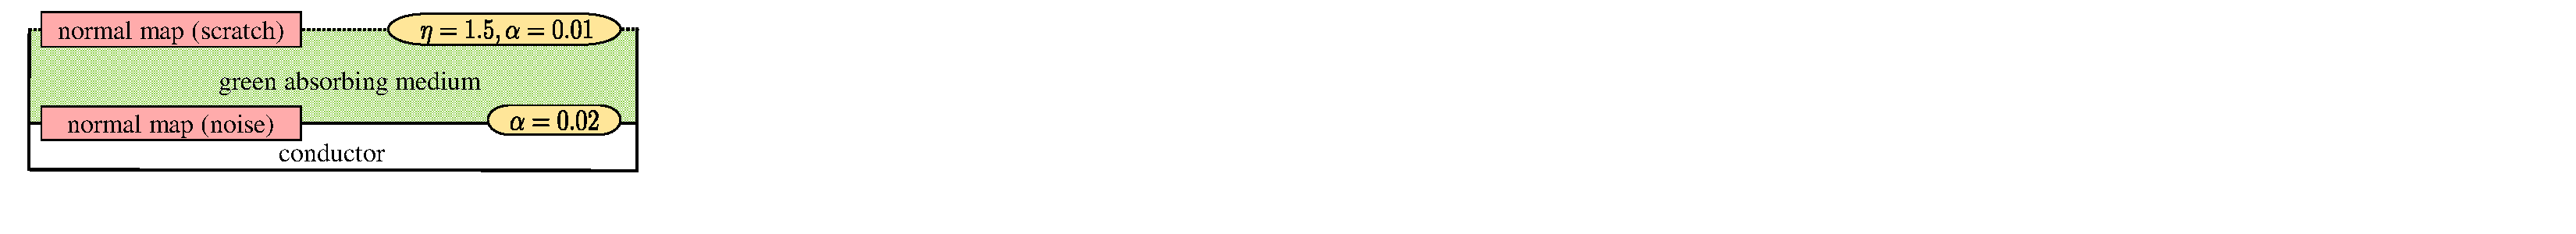
\includegraphics[width=\imgWidth]{layeredbsdf/teaser/green.pdf} &
		
\includegraphics[width=\imgWidth]{layeredbsdf/teaser/yellow.pdf} \\
		\bfseries (b2) & \bfseries (c2) \\
		& \\
		
\includegraphics[width=\imgWidth]{layeredbsdf/teaser/blue.pdf} &
		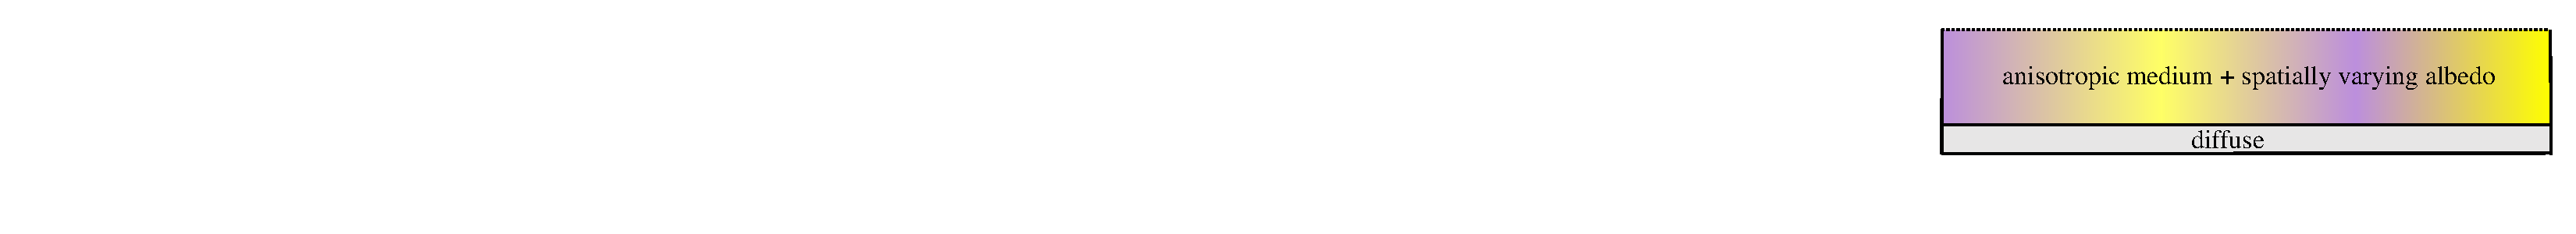
\includegraphics[width=\imgWidth]{layeredbsdf/teaser/magenta.pdf} \\
		\bfseries (d2) & \bfseries (e2)
	\end{tabular}
	\caption{\label{fig:layeredbsdf:teaser}
		We introduce a new BSDF model leveraging an efficient Monte Carlo simulation algorithm applied locally to layered geometries.
		Our model enjoys the flexibility of using arbitrary layer interfaces and internal media and is capable of reproducing a wide variety of appearances.
		This example contains three vases on a tablecloth, all described using our BSDF model (see the insets for layer configurations).
	}
\end{figure}
